Datele volumetrice rezultate prin imagistică medicală sunt aranjate pe o grilă de voxeli într-un sistem cartezian. Datele medicale pot fi obținute prin diverse modalități de scanare, cele mai uzuale fiind radiografia, tomografia computerizată (CT), imagistică prin rezonanță magnetică (RMN) și ultrasunetele. Redarea directă a datelor volumetrice este o metodă de vizualizare eficientă și flexibilă pentru implementarea unei aplicații de redare interactivă. Funcțiile de transfer sunt necesare pentru redarea directă a volumului, deoarece acestea au rolul de a face regiuni de interes vizibile prin atribuirea de proprietăți optice voxelilor, precum culoare și opacitate. Funcțiile de transfer bune permit vizualizarea regiunilor de interes fără ca acestea să fie ascunse de regiuni neimportante. În figura \ref{fig:histogram} ilustrat modul în care pot să difere intensitățile pentru materiale diferite. Această informație poate fi utilizată pentru modelarea unei funcții de transfer care evidențiază numai anumite țesuturi sau materiale în obiectul vizualizat. De obicei funcțiile de transfer sunt unidimensionale, adică acestea transformă în mod direct luminanța în culoare și opacitate, dar există și funcții multidimensionale care pot folosi gradienții datelor sau alte proprietăți ale acestora.

\begin{figure}[!htb]
    \centering
    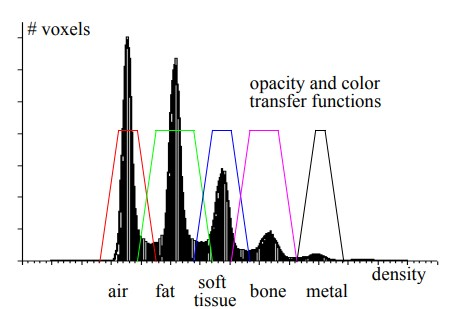
\includegraphics[width=10cm]{images/hist_materials.jpg}
    \\
    \caption{Histogramă a intensităților voxelilor și o clasificare a acestora în diferite materiale. (Sursa imaginii: Kaufman et al. 2005\cite{inbook})}
    \label{fig:histogram}
\end{figure}

Crearea unei funcții de transfer bune poate fi dificilă având în vedere domeniul mare în care poate lua valori luminanța fiecărui voxel. Așadar, explorarea funcției de transfer ar trebui augmentată cu metode suplimentare de vizualizare a datelor, spre exemplu histograme ale densităților în volum. O histogramă a valorilor densității poate fi un indicator util pentru că subliniază structurile dominante cu intervale înguste de densitate\cite{inbook}\cite{rezk2006}. În cazul în care datele conțin zgomot sau sunt reprezentate multe regiuni diferite cu densități similare, poate ajuta și includerea primei derivate în analiza bazată pe histogramă. Valoarea primei derivate (rezistența gradientului) este utilă, deoarece are valori maxime locale la densități în care există schimbări între diferite caracteristici\cite{levoy1988}\cite{inbook}\cite{rezk2006}. Cunoașterea densităților la care există granițele caracteristicilor restrânge considerabil sarcina de explorare a funcției de transfer\cite{inbook}. Funcțiile de transfer multidimensionale folosesc gradientul volumului în timpul redării, adică diferențe centrale pentru a obține vectorul gradient la fiecare voxel. Metoda diferențelor centrale aproximează gradientul ca diferența valorilor datelor a doi voxeli vecini de-a lungul unei axe de coordonate, împărțit la distanța fizică \cite{kniss2002}\cite{rezk2006}. 


O altă modalitate de a analiza datele este căutarea modificărilor topologice în izo-contururile volumului, cum ar fi o îmbinare a două contururi, numite puncte critice. Prin sortarea punctelor critice în funcție de densitate se poate construi un arbore de contur. Se poate folosi arborele de contur fie pentru a genera funcția de transfer automat, sau pentru a ghida utilizatorii în procesul de explorare a volumului \cite{inbook}\cite{Zhou2009AutomaticTF}.


Vizualizarea datelor medicale este dificilă din cauza multitudinii detaliilor de diferite dimensiuni, dar aceasta poate fi simplificată prin evidențierea părților relevante. Tema propusă constă în implementarea și evaluarea unui sistem de redare a unor astfel de date. Integrarea unui mecanism de segmentare semantică a volumelor în procesul de redare permite utilizatorului să vizualizeze regiunile de interes.


\section{Redarea imaginilor medicale}

\textit{Ray casting} a predominat ca abordarea cea mai versatilă pentru redarea directă a datelor volumetrice datorită flexibilității sale în producerea de imagini de înaltă calitate ale seturilor de date medicale și scanărilor industriale \cite{gpugems39}. Datele volumetrice sunt încărcate într-o textură 3D \verb|GL_TEXTURE_3D| și apoi trecute la shader ca un \verb|sampler3D|. Acolo GLSL folosește o funcție de căutare a texturii pentru a obține o valoare de luminanță interpolată liniar.

Modelul ray casting se bazează pe calculul punctelor de intersecție dintre raze și cubul ce conține datele volumului. Pentru fiecare fragment este proiectată o rază dinspre punctul de observare. Se eșantionează iluminarea $I(x,y,z)$ din textură la puncte echidistante de-a lungul razei. Valorile opacității sunt obținute prin interpolare, iar acestea sunt apoi compuse cu fundalul prin compunerea back-to-face pentru a obține culoarea pixelului. Pentru fiecare rază trebuie să determinăm coordonatele punctelor sale de intrare și ieșire în raport cu volumul, acest lucru fiind realizat prin intersecția lor cu un AABB. Acest algoritm este ilustrat în figura \ref{fig:raycasting}.

\begin{figure}[!htb]
    \centering
    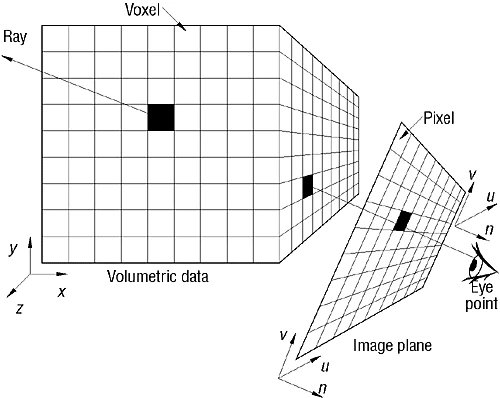
\includegraphics[width=12cm]{images/raycasting.png}
    \\
    \caption{Ilustrare a principiului de funcționare a metodei ray casting de redare a imaginilor volumetrice. (Sursa imaginii: Palmer et al. 1998\cite{palmen1998})}
    \label{fig:raycasting}
\end{figure}

Cea mai simplă tehnică de ray casting este cea în două treceri. Denumirea provine de la faptul că redarea este efectuată în două etape: 

\begin{enumerate}
    \item O primă trecere pentru a calcula geometria limită, adică punctele de intrare și de ieșire ale razelor generate de fiecare pixel din fereastră de vizualizare, redându-le la o textură auxiliară.
    \item O a doua trecere pentru a efectua eșantionarea și compunerea efectivă.
\end{enumerate}

În prima trecere caseta de delimitare a volumului, definită ca un cub de două unități, este redată într-un
 \verb|GL_FRAMEBUFFER|. O transformare a modelului va compensa diferențele de dimensiune dintre axe și orientarea spațială. \verb|GL_FRAMEBUFFER| vă avea două variabile legate de acesta: una va colecta coordonatele spațiale ale punctelor de intrare, date de fața frontală a cubului, cealaltă va colecta punctele de ieșire, date de fața din spate.

Deși este simplu de implementat, tehnica ray casting în două treceri este suboptimă \cite{10.2312:VG:VG06:039-046}. O soluție mai bună este calcularea punctelor de intrare și ieșire ale razelor direct în shaderul fragmentului. Pentru a face acest lucru, trebuie transmise mai multe informații shaderului: poziția camerei (în coordonatele modelului) și câmpul vizual. Ecuația parametrică a razei este:
\begin{equation}
    r = o + tv,
\end{equation}
unde $o$ este originea razei și $v$ este direcția.
În timp ce coordonata sa $z$ este egală în valoare absolută cu distanța focală $f$, aceasta poate fi calculată imediat din câmpul vizual $\alpha$:

\begin{equation}
    f = \frac{1}{tan \frac{\alpha}{2}}.
\end{equation}

Tehnica de redare folosită în acest proiect este compunere alfa back-to-front (din spate în față) descrisa de ecuațiile:
\begin{equation}
    c_i = c_i + (1 - a_i) c_{i+1},
\end{equation}
\begin{equation}
    a_i = a_i + (1 - a_i) a_{i+1},
\end{equation}
unde $c_i$ și $a_i$ reprezintă culoarea și opacitatea pixelului la pasul $i$ din compunere.

Unul dintre motivele importante pentru redare din spate în față este că permite oprirea timpurie a eșantionării atunci când culoarea fragmentului este saturată. Cu toate acestea, nu reduce foarte mult timpul de calcul din cauza naturii paralele ale procesoarelor grafice.

\begin{figure}[!htb]
    \centering
    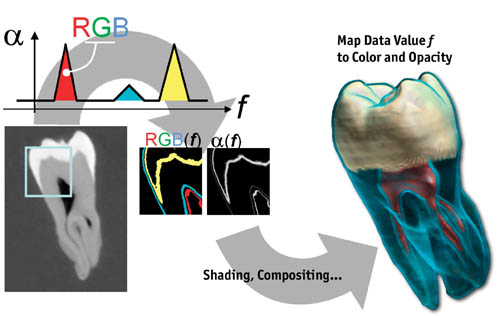
\includegraphics[width=12cm]{images/ilustrare_tf.jpg}
    \\
    \caption{Ilustrare a aplicării funcției de transfer pentru evidențierea materialelor diferite dintr-o scanare CT a unui dinte. (Sursa imaginii: GPU Gems, capitolul 39\cite{gpugems39})}
    \label{fig:ilustr_tf}
\end{figure}

În redarea volumului, funcțiile de transfer \cite{kniss2002} sunt folosite pentru a determina proprietățile voxelului în culoare și opacitate folosind valorile luminanței. Pentru a reprezenta structura unei entități înglobate într-un volum este necesară eliminarea structurilor nedorite, care ascund regiunile de interes. Acest lucru este de obicei realizat printr-o funcție de transfer care mapează valorile dintr-un set de date la anumite culori și opacități. O definiție de bază a unei funcții de transfer, $T$, este exprimată ca:
\begin{equation}
    c = T(i),
\end{equation}
unde $i$ este intensitatea punctului curent. Pe urmă aceste date vor fi folosite în tehnica de compunere alfa back-to-front prezentată mai sus. Un exemplu de aplicare a unei astfel de funcții poate fi regăsit în figura \ref{fig:ilustr_tf}.

Rata de eșantionare poate fi scăzută în timpul interacțiunii utilizatorului cu volumul, adică în timpul aplicării transformărilor de rotație, translație și scalare, astfel crescând numărul de cadre redate pe secundă pe sistemele cu performanțe mai scăzute, făcând mai ușoară încadrarea în fereastra de redare a regiunilor de interes. Atunci când rata de eșantionare este scăzută, detaliile obiectului vizualizat vor dispărea, dar forma generală a acestuia va rămâne. După ce a fost încadrat obiectul, rata de eșantionare poate fi crescută pentru a obține o imagine mai detaliată, după cum poate fi observat într-un exemplu în figura \ref{fig:sample_rate}. 

\begin{figure}[!htb]
    \centering
    \captionsetup{justification=centering}
    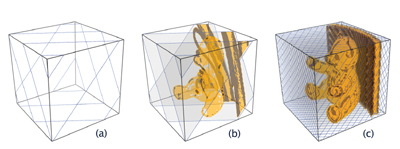
\includegraphics[width=10cm]{images/sample_rate.jpg}
    \\
    \caption{Ilustrare a redării volumului folosind rate de esantioare diferite. Rata de eșantionare crește progresiv în imagini de la stangă la dreapta.
    \\
    (a) - rata de eșantionare prea mică pentru a fi observabil obiectul;
    \\
    (b) - rata de eșantionare suficient de mare pentru observarea structurii obiectului;
    \\
    (c) - rata de eșantionare suficient de mare pentru observarea detaliilor obiectului
    \\
    (Sursa imaginii: GPU Gems, capitolul 39\cite{gpugems39})}
    \label{fig:sample_rate}
\end{figure}

Clipping-ul este o tehnică fundamentală de interacțiune pentru a explora datele volumetrice medicale. Această tehnică este folosită pentru a restricționa vizualizarea la subvolume. În timp ce funcțiile de transfer restricționează vizualizarea la acele părți care au anumite proprietăți (valori de intensitate, gradienți) în comun, clippingul exclude anumite forme geometrice din vizualizare. Planurile de tăiere sunt translate de utilizator, iar vizualizarea este actualizată continuu. Combinația de șase planuri de tăiere poate fi utilizată pentru a defini un subvolum.


\section{Lucrări similare}

\begin{figure}[!htb]
    \centering
    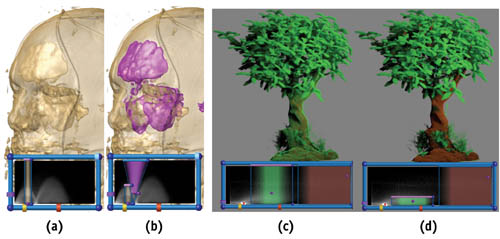
\includegraphics[width=12cm]{images/2d_tf.jpg}
    \\
    \caption{Diferență dintre funcții de transfer unidimensionale ((a) și (c)) și multidimensionale ((b) și (d)). (Sursa imaginii: GPU Gems, capitolul 39\cite{gpugems39})}
    \label{fig:ilustr_2dtf}
\end{figure}

Autorii lucarii \cite{kniss2002} prezintă posibile modalități de utilizare a funcțiilor de transfer multidimensionale într-o aplicație de vizualizare a datelor medicale volumetrice. Pentru creerea acestui tip de funcții este prezentat un widget ce permite utilizatorului să modifice o funcție de transfer în două dimensiuni: intensitatea voxelilor și magnitudinea gradientului obținut prin diferențe centrale. Autorii acestei lucrări susțin că funcțiile de transfer multidimensionale sunt eficiente pentru vizualizarea granițelor dintre diferite regiuni ale volumului de date analziat și diferite materiale în acesta. De asemenea, acest tip de funcții poate fi folosit pentru izolarea anumitor proprietăți din volum, după cum poate fi observat și în figura \ref{fig:ilustr_2dtf}.

\begin{figure}[!htb]
    \centering
    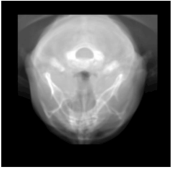
\includegraphics[width=5cm]{images/fvr_a.png}
    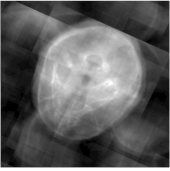
\includegraphics[width=5cm]{images/fvr_b.png}
    \\
    \caption{Rezultatul redării unei scanări computer tomograf a unui cap folosind tehnica redării prin metoda Fourier. În stânga proiecția este ortogonală, iar în dreapta este rotită, observându-se artefacte. (Sursa imaginii: Abdellah et al.2015 \cite{abdellah2015})}
    \label{fig:fvr}
\end{figure}

Redarea volumului prin metoda Fourier (FVR) este o tehnică de vizualizare care a fost utilizată pe scară largă în radiografia digitală. Ca rezultat al complexității în timp O($N^2 log N$), oferă o alternativă mai rapidă la algoritmii de redare a volumului din domeniul spațial care sunt complecși din punct de vedere computațional O($N^3$). Introducerea tehnologiei compute unified device architecture (CUDA) permite algoritmilor paraleli să ruleze eficient pe arhitecturile GPU compatibile CUDA. În  \cite{abdellah2015} este prezentată o implementare accelerată de GPU de înaltă performanță a metodei FVR pe GPU-uri folosind CUDA. Această implementare poate obține o accelerare de 117x în comparație cu o implementare hibridă cu un singur thread care utilizează CPU și GPU împreună \cite{abdellah2015}. Cu toate că redarea este obținută considerabil mai rapid decât cu redarea directă a volumelor, rezultatul nu este la fel de calitativ, conținând artefacte în unele cazuri, după cum poate fi observat și în figura \ref{fig:fvr}.

În \cite{radiuk2020} sunt investigate rețelele neuronale complet convoluționale (FCN\footnote{FCN sau fully convolution network este o rețea neuronală în care singurele operație efectuată sunt cele de convoluție și agregare.}) și se propune o arhitectură UNet 3D dedicată procesării imaginilor volumetrice obținute prin tomografie computerizată în scopul segmentării semantice automate. A fost comparată arhitectura propusă în lucrare cu mai multe metode și a fost arătat că arhitecturile bazate pe UNet 3D pot obține performanțe ridicate în sarcinile de segmentare multi-organe folosind un singur GPU. Abordarea propusă a segmentării imaginii 3D nu implică nicio restricție asupra formei anatomiei segmentate. Această omisiune poate duce la zone izolate la marginile organelor. De exemplu, redarea 3D detaliază slab imaginile părților subțiri ale corpului cu puțini voxeli, cum ar fi arterele și venele.

Parametrii stratului convoluțional constau dintr-un set de filtre care pot fi învățate. Fiecare filtru este mic din punct de vedere spațial. În timpul inferenței, fiecare filtru este glisat pe fiecare dimensiune a volumului de intrare și este calculat produsul între intrările filtrului și intrarea în orice poziție în spațiul intrării. Rețeaua va învăța filtre care se activează atunci când identifică un anumit tip de caracteristică vizuală, cum ar fi o margine cu anumită orientare \cite{cs231n}.

Pentru rețeaua UNet sunt folosite în codificator straturi convolutionale cu filtre de 3 × 3 × 3 urmate de funcții de activare de tip Rectified Linear Unit (ReLU)\cite{DBLP:journals/corr/abs-1803-08375} și agregarea de tip Max Pooling de 2 × 2 × 2. In mod uzual in retelele UNet intre codificator și decodor este un strat complet conectat (fully connected, FC) numit bottleneck. În arhitectura prezentată de autorii lucrării \cite{radiuk2020}, in loc de un strat complet conectat este folosit un bloc convoluțional. Decodorul conține straturile convoluționale transpuse 3 × 3 × 3 ca straturi finale, fiecare dintre ele utilizând activări ReLU. După stratul convoluțional final, se aplică o funcție de activare sigmoid cu un prag pentru a determina etichetele de segmentare semantică de ieșire \cite{radiuk2020}. Arhitectura descrisă mai sus este ilustrată în figura \ref{fig:UNet}. În arhitectura din figură numărul de filtre pentru fiecare bloc convoluțional este o putere consecutivă a lui 2 începând de la 64, adică: primul bloc conține două straturi convoluționale, fiecare având 64 filtre, în următorul bloc straturile au 128 filtre, continuând până la blocul convoluțional bottleneck care are 1024 filtre.

\begin{figure}[!htb]
    \centering
    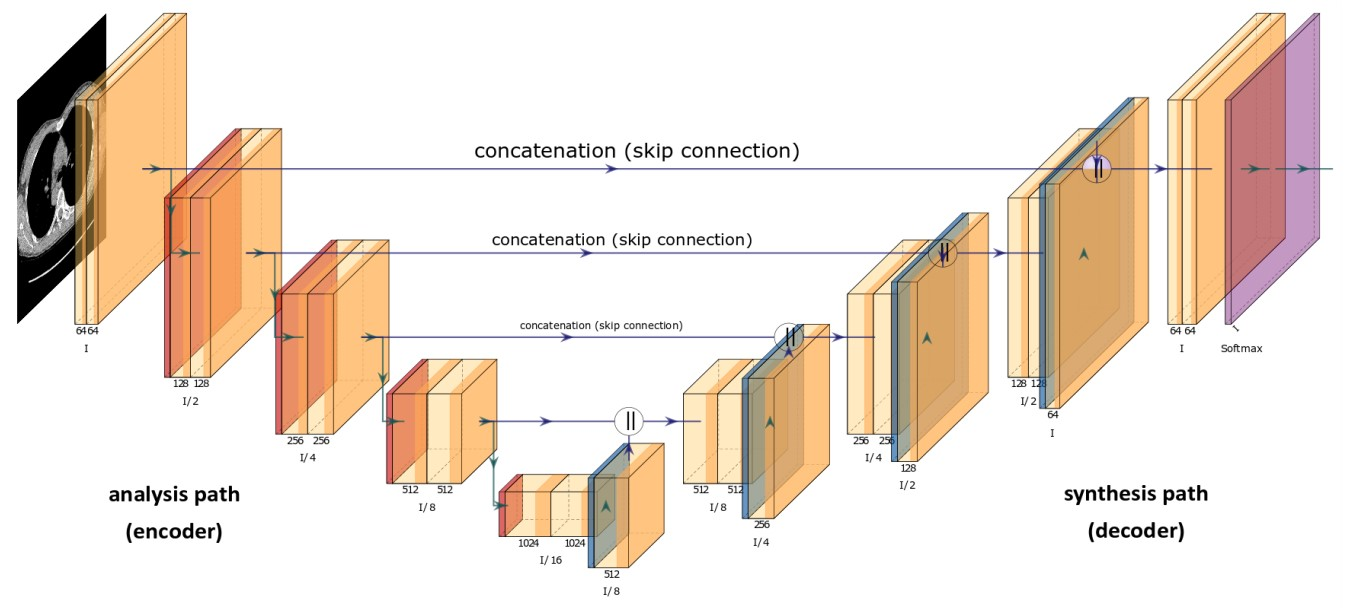
\includegraphics[height=7.5cm]{images/schema_UNET_radiuk.jpg}
    \\
    \caption{Arhitectura U-Net 3D. (Sursa imaginii: Radiuk et al. 2020\cite{radiuk2020})}
    \label{fig:UNet}
\end{figure}

Autorii lucrării \cite{sequential2019} prezinta o arhitectură similară cu UNet 3D, diferența principală fiind faptul că bottleneck-ul și rețeaua convoluțională finală sunt înlocuite de rețele recurente bidirecționale. Autorii propun o metodă prin care segmentarea este efectuată felie după felie din volumul de date, astfel reducându-se cerințele de memorie și durata efectuării retropropagării.

În \cite{weiss2021deep} este propusă o metodă de redare a imaginilor volumetrice folosind rețele neuronale. Metoda propusă, numită DeepDVR, poate învăța să redea imagini volumetrice în care regiunile de interes sunt vizibile și clar delimitate fară să fie necesară creerea unei funcții de transfer, care este o operație costisitoare pentru utilizator. Modelul prezentat a fost antrenat pe un set de date ce conținea predominant imagini cu o calitate scăzută, dar atunci când acesta a fost testat pe date cu calitate înaltă, a generat redări promițătoare. Arhitectura este, din nou, bazată pe UNet 3D, diferența principală fiind faptul că au fost înlocuite conexiunile între blocurile convoluționale și cele convoluționale transpuse cu un modul nou, iar bottleneck-ul a fost eliminat pentru a permite dimensiunea volumului de intrare să fie arbitrară și dimensiunea ieșirii să fie diferită față de cea de intrare. Este de notat faptul că această rețea primește o intrare tridimensională și ieșirea vă fi bidimensională, așadar modulele dintre codificatoare și decodificatoare vor avea un rol important în abstractizarea corectă a informațiilor.

Pentru aplicarea unei rețele neuronale într-o aplicație, dimensiunea acestora trebuie să fie redusă deoarece este de dorit ca rezultatul să fie obținut cât mai rapid. În acest sens sunt explorate rețele neuronale de dimensiuni reduse. O alternativă a reducerii dimensiunii rețelei este învățarea prin transfer \cite{chen2019med3d}.
